\section{Experimental Results \label{sec:evaluation}}




\subsection{Performance on \TimeRE} \label{sec:results_in_TimeRE}
\begin{figure}[t!]
% \begin{figure}[htbp]
% \setlength{\abovecaptionskip}{3pt}
\setlength{\belowcaptionskip}{-10pt}
\begin{center}
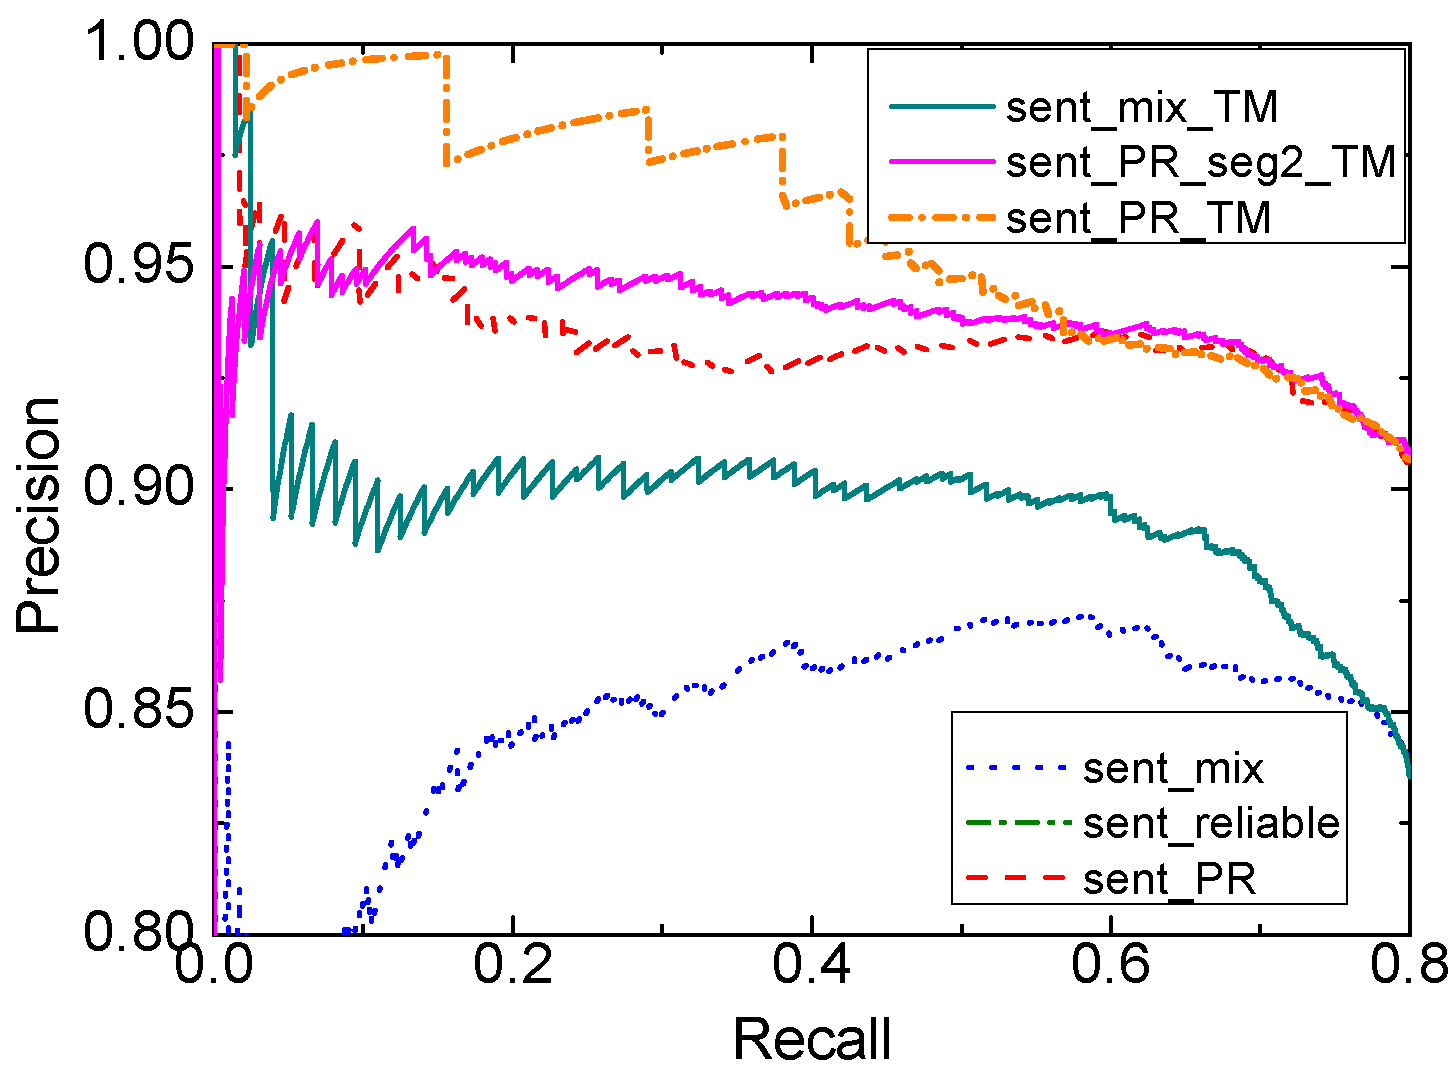
\includegraphics[width=0.45\textwidth]{figures/sent_time_exp_overall.pdf}
\caption{Sentence Level Results on \TimeRE}
\label{fig: sent_luo}
\end{center}
\end{figure}

\paragraph{Sentence Level Models}
The results of sentence level models on \TimeRE are shown in Figure \ref{fig:
sent_luo}. We can see that mixing all subsets together (\texttt{sent\_mix})
gives the worst performance,  significantly
worse than using the reliable subset only (\texttt{sent\_reliable}). This
suggests the noisy nature of the training data obtained through \DS and
properly dealing with the noise is the key for \DS for a wider range of applications. %to be adopted at a wider scale.
When getting help from our dynamic transition matrix, % during training, the
the model (\texttt{sent\_mix\_TM}) significantly improves \texttt{sent\_mix},
delivering the same level of performance as \texttt{sent\_reliable} in most
cases. This suggests that our transition matrix can help to mitigate the bad influence of noisy training instances.


Now let us consider the \texttt{PR} scenario where one can build a curriculum by first training on the
reliable subset, then gradually moving to both reliable and less
reliable data. We can see that, this simple curriculum learning based model
(\texttt{sent\_PR}) further outperforms \texttt{sent\_reliable} significantly,
indicating that the curriculum learning framework not only reduces the effect
of noise, but also helps the model learn from noisy data. When applying the
transition matrix approach into this curriculum learning framework using one reliable
subset and one unreliable subset generated by mixing our two less reliable subsets, our model (\texttt{sent\_PR\_seg2\_TM})
further improves \texttt{sent\_PR} by  %exploring the prior knowledge about data quality and
utilizing the dynamic transition matrix to model the noise.
%enabling the transition matrix approach to control the noise at different levels during different curriculums. }
% \todo{ZW: Have no idea of what this sentence is talking about. \textbf{I have rephrased it}.}
% (\orange{I further rephrased this sentence.})
It is not surprising that when we use all three subsets separately,
our model (\texttt{sent\_PR\_TM}) significantly outperforms all
other models by a large margin.
%\footnote{We will use all three subsets separately for all \texttt{\_PR} settings in the rest of the experiments.}.

\begin{figure*}[t!]
% \begin{figure*}[htbp]
% \setlength{\abovecaptionskip}{3pt}
\setlength{\belowcaptionskip}{-10pt}
\centering
\subfigure[Attention Aggregation]{
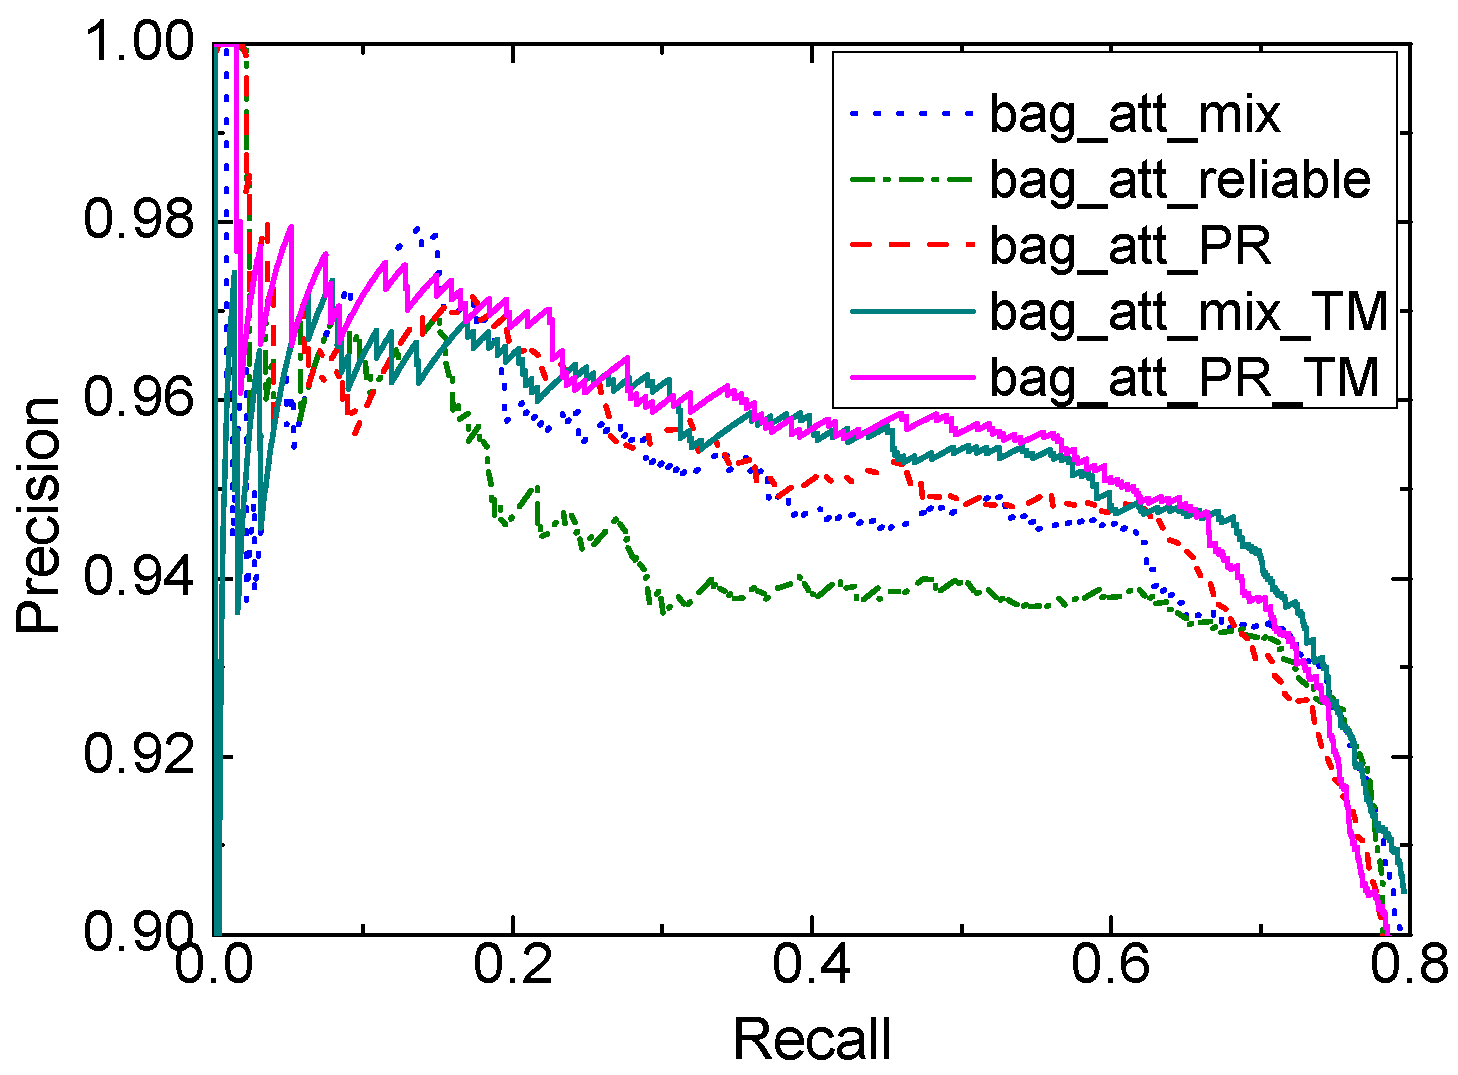
\includegraphics[width=0.45\textwidth]{figures/bag_att_exp_overall.pdf}
\label{fig: bag_att_luo}
}
\subfigure[Average Aggregation]{
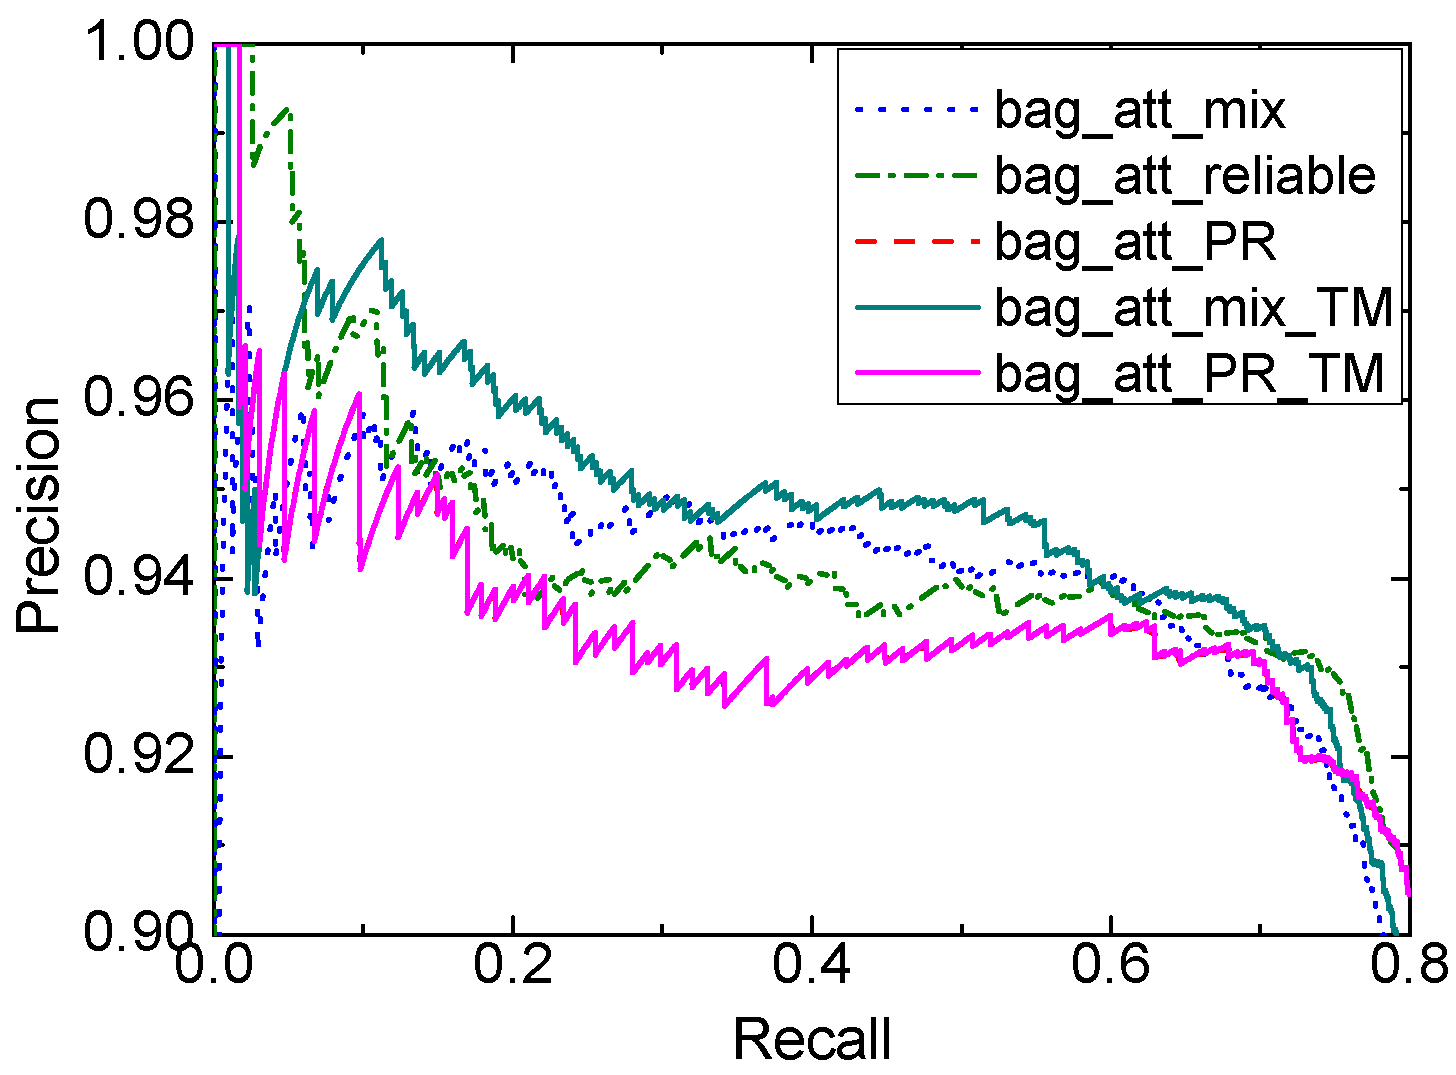
\includegraphics[width=0.45\textwidth]{figures/bag_avg_exp_overall.pdf}
\label{fig: bag_avg_luo}
}
\caption{Bag Level Results on \TimeRE}
\label{fig: results_on_luo}
\end{figure*}


\paragraph{Bag Level Models}
In this setting, we first look at the performance of the bag level models with attention aggregation. The results are shown in Figure~\ref{fig: bag_att_luo}.
Consider the comparison between the  model trained on the reliable subset only (\texttt{bag\_att\_reliable}) and the one trained on the mixed dataset (\texttt{bag\_att\_mix}).
In contrast to the sentence level, \texttt{bag\_att\_mix} outperforms \texttt{bag\_att\_reliable} by a large margin, because \texttt{bag\_att\_mix} has taken the \textit{at-least-one assumption} into consideration through the attention aggregation mechanism (Eq.~\ref{att_sum}), which can be seen as a denoising step within the bag.
This may also be the reason that when we introduce either our dynamic transition matrix (\texttt{bag\_att\_mix\_TM})  or the curriculum of using prior knowledge of data quality (\texttt{bag\_att\_PR}) into the bag level models, the improvement regarding \texttt{bag\_att\_mix}  is not as significant as in the sentence level.

However, when we apply our dynamic transition matrix %to model the noise with
into the curriculum built upon prior knowledge of data quality (\texttt{bag\_att\_PR\_TM}), the performance gets further improved. This happens especially in the high precision part compared to \texttt{bag\_att\_PR}.
We also note that the bag level's \textit{at-least-one assumption} does not always hold, and there are still false negative and false positive problems. Therefore, using our transition matrix approach with or without prior knowledge of data quality, i.e., \texttt{bag\_att\_mix\_TM}  and \texttt{bag\_att\_PR\_TM}, both improve the performance, and \texttt{bag\_att\_PR\_TM} performs slightly better.

%\paragraph{Bag Level Average Aggregation Models}

%As shown in Figure~\ref{fig: bag_avg_luo}, the relative ranking of various settings in the bag level models with average aggregation is similar to those with attention aggregation.
The results of bag level models with average aggregation are shown in Figure \ref{fig: bag_avg_luo}, where the relative ranking of various settings is similar to those with attention aggregation.
A notable difference is that both \texttt{bag\_avg\_PR} and \texttt{bag\_avg\_mix\_TM} improve \texttt{bag\_avg\_mix} by a larger margin compared to that in the attention aggregation setting. The reason may be that the average aggregation mechanism is not as good as the attention aggregation in denoising within the bag, which leaves more space for our transition matrix approach or curriculum learning with prior knowledge to improve.
Also note that \texttt{bag\_avg\_reliable} performs best in the very-low-recall region but worst in general.
This is because that it ranks higher the sentences expressing either \texttt{birth-date} or \texttt{death-date}, the simplest but the most common relations in the dataset, but fails to learn other relations with limited or noisy training instances, given its relatively simple aggregation strategy.
%. However, due to the less amount of data, this model performs worse in other relations and thus generates the worst results in general.
% Therefore, this shows that training only on the reliable data leads the model to use the most common patterns with high confidence, but the less amount of data makes it performs worse in general.
%\red{why (\texttt{bag\_avg\_reliable}) performs so much better than all others in the very high precision stage ($recall<0.05$)?????????}
%\orange{Another prominent difference lies in the performance drop of \emph{bag\_avg\_PR\_TM} in the low-recall area ($recall<0.15$). With manual investigation, we find that this is caused by some high ranking of false negative data}
%However, since  denoising ability is not as good as attention aggregation, adding unreliable data gradually (\emph{bag\_avg\_currd}) improves the model performance here. We can also see that the transition matrix improves the average aggregation models more significantly than the attention aggregation models.
 %Note that due to the inferior denoising ability of average aggregation, the unhandled sentence level noise may further propagates to bag level, which gives the transition matrix more chance to help model the noise.

% \begin{table}
% \centering
% \small{
% \begin{tabular}{|c|c|c|c|c|}
% \hline
% % \textbf{Att\_Weight}
% % \bm{$\beta$}
% \textbf{Method}							& \textbf{P@R\_10} 		& \textbf{P@R\_30} 			& \textbf{P@R\_50} \\
% \hline
% \textit{sent\_mix} 						&80.81	&84.98	&86.90 	\\
% \hline
% \textit{sent\_mix\_TM} 				&89.39	&90.24	&90.23 	\\
% \hline
% \textit{sent\_PR} 						&94.24	&93.06	&93.27 	\\
% \hline
% \textit{sent\_PR\_TM} 				&\textbf{99.64}	&\textbf{97.42}	&94.74 	\\
% \hline
% \textit{bag\_avg\_mix} 				&95.53	&94.87	&94.09 	\\
% \hline
% \textit{bag\_avg\_mix\_TM} 		&97.54	&94.87	&94.80 	\\
% \hline
% \textit{bag\_avg\_PR} 				&96.86	&95.19	&94.61 	\\
% \hline
% \textit{bag\_avg\_PR\_TM} 			&97.20	&95.85	&95.32 	\\
% \hline
% \textit{bag\_att\_mix} 				&97.20	&95.30	&94.80 	\\
% \hline
% \textit{bag\_att\_mix\_TM} 		&96.53	&96.18	&95.45 	\\
% \hline
% \textit{bag\_att\_PR} 				&95.86	&95.63	&94.87 	\\
% \hline
% \textit{bag\_att\_PR\_TM} 			&97.19	&95.96	&\textbf{95.65} 	\\
% \hline
% \end{tabular}
% }
% \caption{\orange{Overall comparison on \TimeRE. P@R\_10/30/50 refers to the precision when recall equals 10\%, 30\%, and 50\%.}}
% \label{overall_TimeRE}
% \end{table}

% \paragraph{Sentence Level v.s. Bag Level}
% \orange{We summarize the performances of the sentence level and bag level models in Table~\ref{overall_TimeRE}.} We can see that, since the \textit{at-least-one assumption} alleviates the noisy data problem, bag level models performs better than sentence level models when no prior knowledge about data quality is used (\texttt{\_mix}). Even with the powerful transition matrix, \texttt{sent\_mix\_TM} still performs worse than \texttt{bag\_att\_mix}, indicating the importance of good observations about the dataset. However, when we divide the dataset into several subsets with different reliability levels (\texttt{\_PR}), \texttt{sent\_PR\_TM} performs generally better than bag level models.
% This shows that, with proper guidance, using transition matrix to model the sentence level noise is better than using the \textit{at-least-one assumption} to transform the fine-grained sentence level noise to the coarse bag level noise.



\paragraph{Global v.s. Dynamic Transition Matrix}
\begin{figure}[t!]
% \setlength{\abovecaptionskip}{3pt}
% \setlength{\belowcaptionskip}{-10pt}
\begin{center}
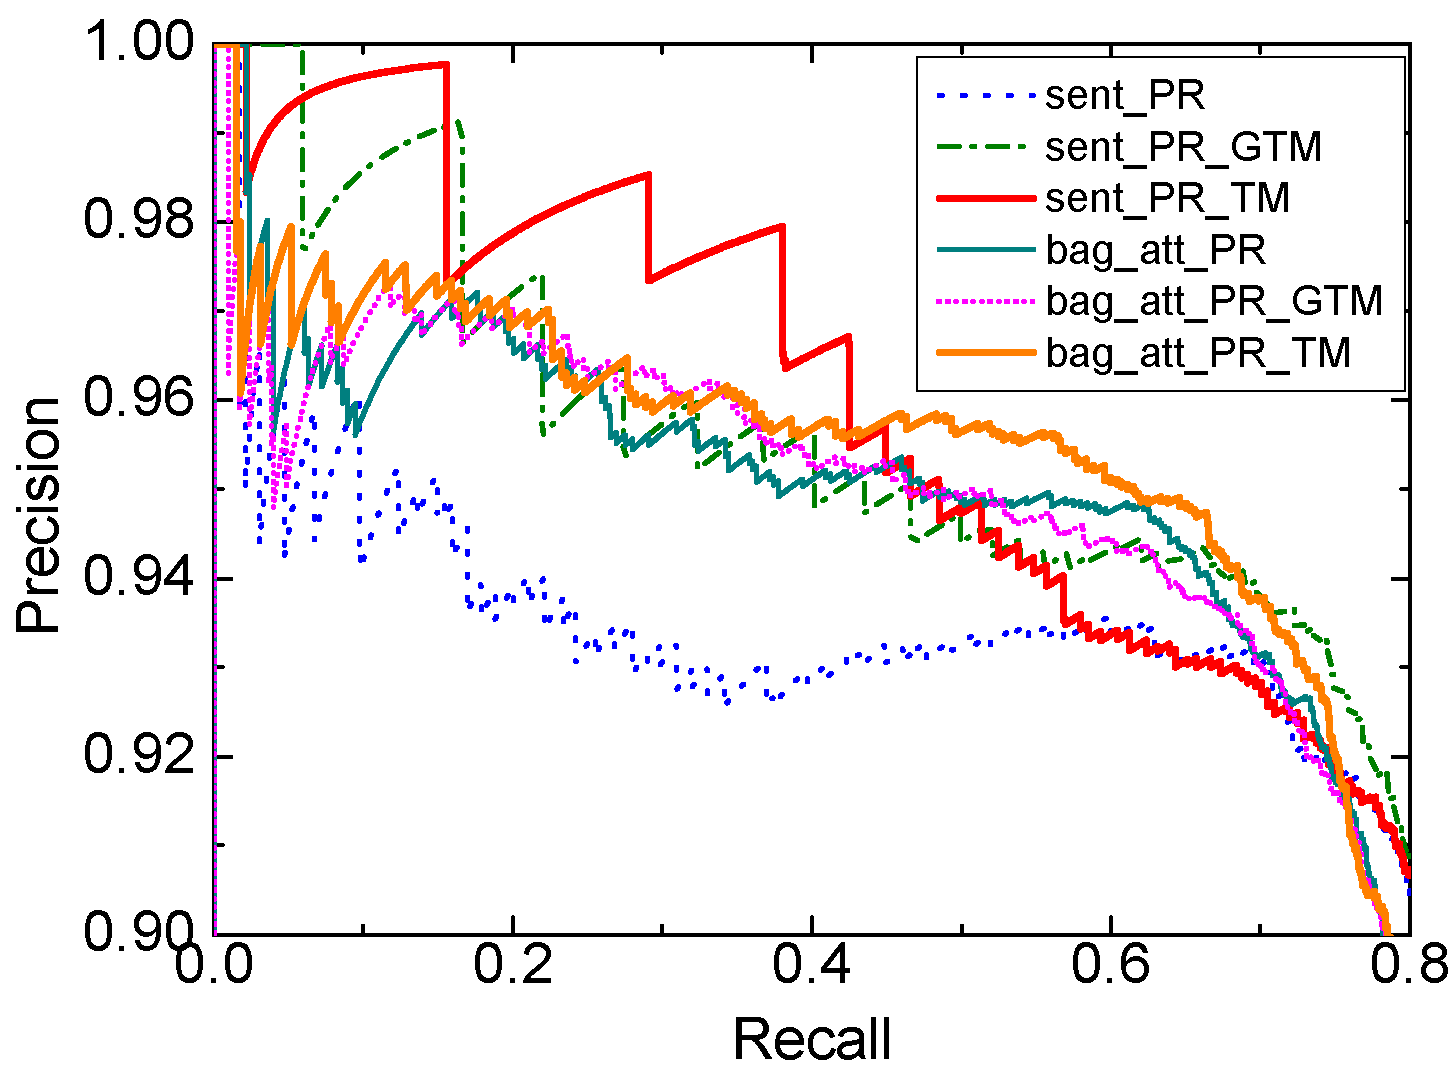
\includegraphics[width=0.45\textwidth]{figures/single_cmp_exp_overall.pdf}
\caption{Global TM v.s. Dynamic TM}
\label{fig: cmp_single_dynamic}
\end{center}
\end{figure}
We also compare our dynamic transition matrix method with the global transition matrix method,
which maintains only one transition matrix for all training instances. %instead of dynamically producing a transition matrix for each instance.
% and is updated via back-propagation during training. 
\orange{Specifically, instead of dynamically generating a transition matrix for each datum, we first initialize an identity matrix $\mathbf{T}'\in\mathbb{R}^{|\mathbb{C}|\times |\mathbb{C}|}$, where $|\mathbb{C}|$ is the number of relations (including \texttt{no-relation}).
Then the global transition matrix $\mathbf{T}$ is built by applying \emph{softmax} to each row of $\mathbf{T}'$ so that $\sum_j{\mathbf{T}_{ij}}=1$:}
\begin{equation}
\label{shared_mat}
T_{ij} = \frac{e^{T'_{ij}}}{\sum_{j=1}^{|\mathbb{C}|}{e^{T'_{ij}}}}
\end{equation}
where $T_{ij}$ and $T'_{ij}$ are the elements in the $i^{th}$ row and $j^{th}$ column of $\mathbf{T}$ and $\mathbf{T}'$. The element values of matrix $\mathbf{T}'$ are also updated via backpropagation during training.
As shown in Figure~\ref{fig: cmp_single_dynamic},
%we can see that 
using one global transition matrix (\texttt{\_GTM}) is also beneficial and improves both the sentence level (\texttt{sent\_PR}) and bag level  (\texttt{bag\_att\_PR}) models. However, since the global transition matrix only 
captures the global noise pattern, it fails to characterize individuals with subtle differences, 
resulting in a performance drop compared to the dynamic one (\texttt{\_TM}).


\paragraph{Case Study}
\orange{We find our transition matrix method tends to obtain more significant improvement on noisier relations.} For example, \textit{time\_of\_spacecraft\_landing} is noisier than \textit{time\_of\_spacecraft\_launch} since compared to the launching of a spacecraft, there are fewer sentences containing the landing time of a spacecraft that talks directly about the landing. Instead, many of these sentences tend to talk about the activities of the crew. Our \texttt{sent\_PR\_TM} model improves the F1 of \textit{time\_of\_spacecraft\_landing} and \textit{time\_of\_spacecraft\_launch} over \texttt{sent\_PR} by 9.09\% and 2.78\%, respectively. 
The transition matrix makes more significant improvement on \textit{time\_of\_spacecraft\_landing} since there are more noisy sentences for our method to handle, which results in more significant improvement on the quality of the training data.


\subsection{Performance on \EntityRE}
We evaluate our bag level models on \EntityRE.
As shown in Figure~\ref{fig: Riedel_res}, it is not surprising that the basic model with attention aggregation (\texttt{att}) significantly outperforms the average one (\texttt{avg}), where \texttt{att}  in our bag embedding is similar in spirit to \cite{lin2016neural},
which has reported the-state-of-the-art performance on \EntityRE.
When injected with our transition matrix approach,  both \texttt{att\_TM} and \texttt{avg\_TM} clearly outperform their basic versions.

%since the unhandled sentence level noise propagates to the bag level, which makes the bag level noise become more severe, the transition matrix has more chance to model the noise. Therefore, the \emph{avg\_TM} model clearly outperforms the \emph{avg} model.
Similar to the situations in \TimeRE, since \texttt{att} has taken the \textit{at-least-one assumption} into account  through its attention-based bag embedding mechanism, thus the improvement by \texttt{att\_TM}  is not as large as by \texttt{avg\_TM}.
%Since
%Note that the low recall part corresponds to high precision, which is more useful than the rest of the extraction results in practice. Therefore, our transition matrix method is also useful in this situation.

\begin{figure}[t!]
% \begin{figure}[htbp]
% \setlength{\abovecaptionskip}{3pt}
% \setlength{\belowcaptionskip}{-10pt}
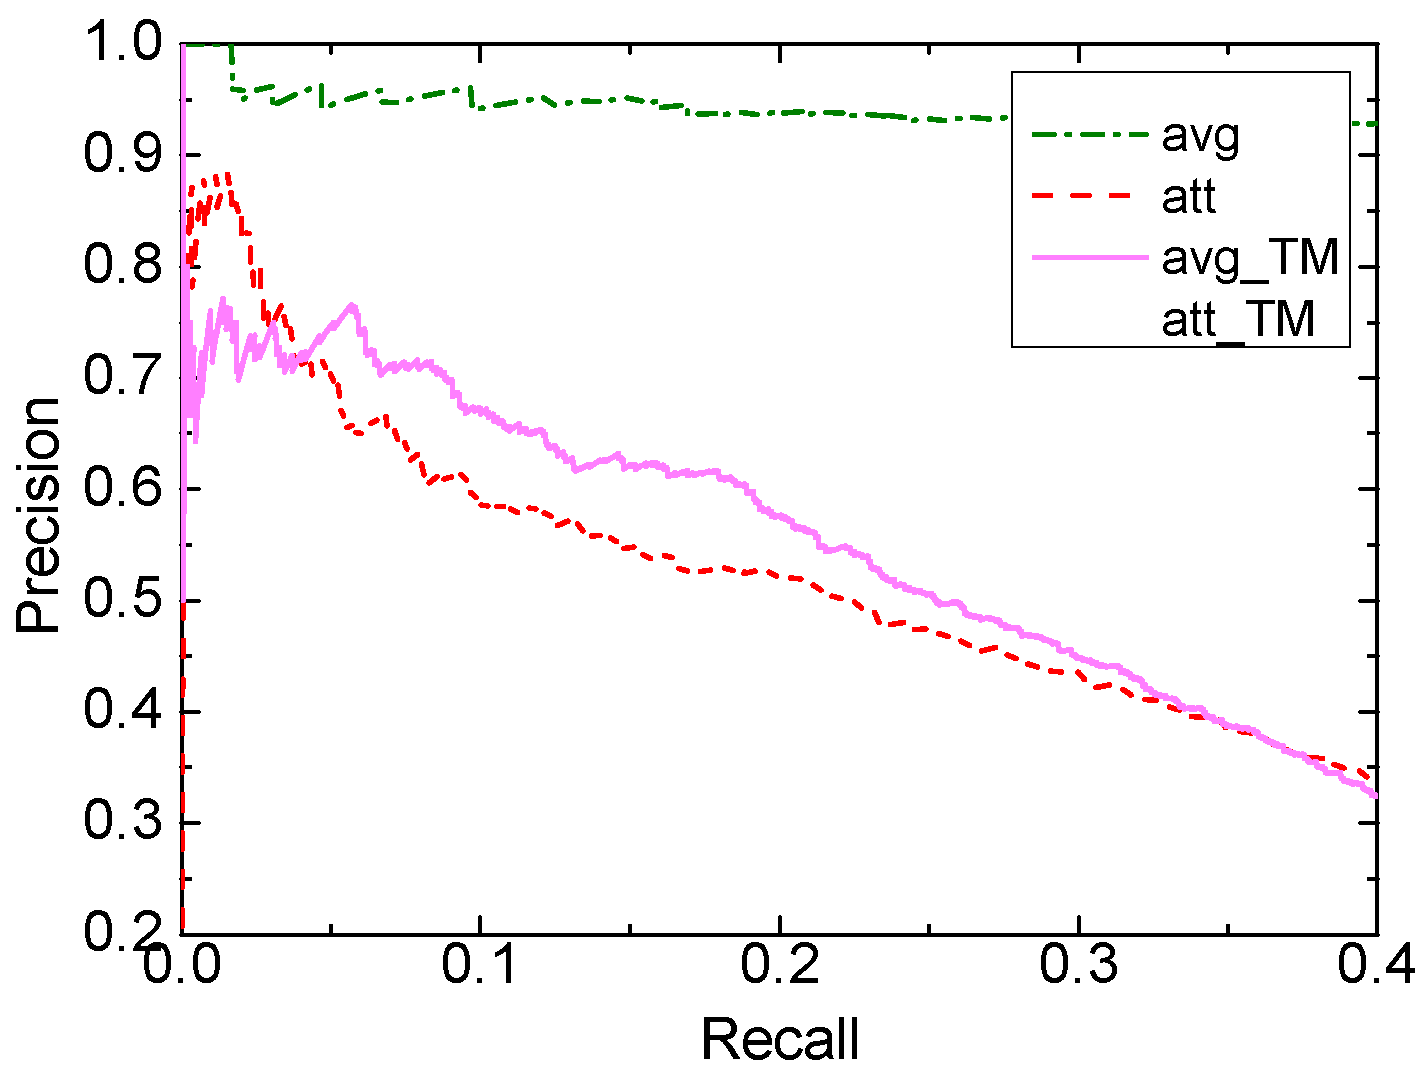
\includegraphics[width=0.45\textwidth]{figures/re_att_avg_cmp_exp.pdf}
\caption{Results on \EntityRE}
\label{fig: Riedel_res}
\end{figure}



\begin{table}
\centering
\small{
\begin{tabular}{|c|c|c|c|c|c|}
\hline
% \textbf{Att\_Weight}
% \bm{$\beta$}
\textbf{Method}							& \textbf{P@R\_5} 		& \textbf{P@R\_10} 			& \textbf{P@R\_15} & \textbf{P@R\_20} \\
\hline
\textit{Mintz} 							&52.13	&39.88	&34.07	&28.55 	\\
\hline
\textit{MultiR} 						&63.23	&60.94	&41.18	&36.41 	\\
\hline
\textit{MIML} 							&68.53	&60.75	&46.36	&33.82 	\\
\hline
\textit{avg} 								&59.76	&58.04	&54.16	&51.25 	\\
\hline
\textit{avg\_TM} 						&70.50	&58.56	&54.77	&52.35 	\\
\hline
\textit{att} 								&66.67	&61.51	&59.31	&56.36 	\\
\hline
\textit{att\_TM} 						&\textbf{74.81}	&\textbf{67.24}	&\textbf{62.21}	&\textbf{57.61} 	\\
\hline
\end{tabular}
}
\caption{\orange{Comparison with feature-based methods. P@R\_5/10/15/20 refers to the precision when recall equals 5\%, 10\%, 15\% and 20\%.}}
\label{feature-based}
\vspace{-1em}
\end{table}

% \begin{table}
% \centering
% \small{
% \begin{tabular}{|c|c|c|c|c|}
% \hline
% % \textbf{Att\_Weight}
% % \bm{$\beta$}
% \textbf{Method}							& \textbf{P@R\_10} 		& \textbf{P@R\_20} 			& \textbf{P@R\_30} \\
% \hline
% \textit{Mintz} 							&39.88	&28.55	&16.81 	\\
% \hline
% \textit{MultiR} 						&60.94	&36.41	&- 	\\
% \hline
% \textit{MIML} 							&60.75	&33.82	&- 	\\
% \hline
% \textit{avg} 								&58.04	&51.25	&42.45 	\\
% \hline
% \textit{avg\_TM} 						&58.56	&52.35	&43.59 	\\
% \hline
% \textit{att} 								&61.51	&56.36	&\textbf{45.63} 	\\
% \hline
% \textit{att\_TM} 						&\textbf{67.24}	&\textbf{57.61}	&44.90 	\\
% \hline
% \end{tabular}
% }
% \caption{\orange{Comparison with feature-based methods. P@R\_5/10/15/20 refers to the precision when recall equals 5\%, 10\%, 15\% and 20\%.}}
% \label{feature-based}
% \end{table}

% \paragraph{Comparison with Feature-based Methods}
\orange{We also include the comparison with three feature-based methods}: \texttt{Mintz}~\cite{mintz2009distant} is a multiclass logistic regression model; \texttt{MultiR}~\cite{hoffmann2011knowledge} is a probabilistic graphical model that can handle overlapping relations; \texttt{MIML}~\cite{surdeanu2012multi} is also a probabilistic graphical model but operates in the multi-instance multi-label paradigm. As shown in Table~\ref{feature-based}, although traditional feature-based methods have reasonable results in the low recall region, their performances drop quickly as the recall goes up, and \texttt{MultiR} and \texttt{MIML} did not even reach the 30\% recall. This indicates that, while the patterns captured by feature based models are reliable, their coverage is relatively low. On the other hand, neural network models have more stable performance across different recalls, 
and \texttt{att\_TM} performs consistently better than other models,
% and \texttt{att\_TM} performs generally better than other models, 
indicating again the effectiveness of our transition matrix method.






